\section{Motor and Gearing selection}

Selecting the gearbox will change the overall transfer function of the plant, as it modifies components inside the plant. Changing the gearing ratio of the motor adjusts the effective motor torque, similar to changing the motor itself. Gearing ratios were experimented with in order to determine their true effects on the system, while keeping controller poles and zeros fixed (they had already been roughly determined at this point.)

\begin{figure}[ht]
	\centering
		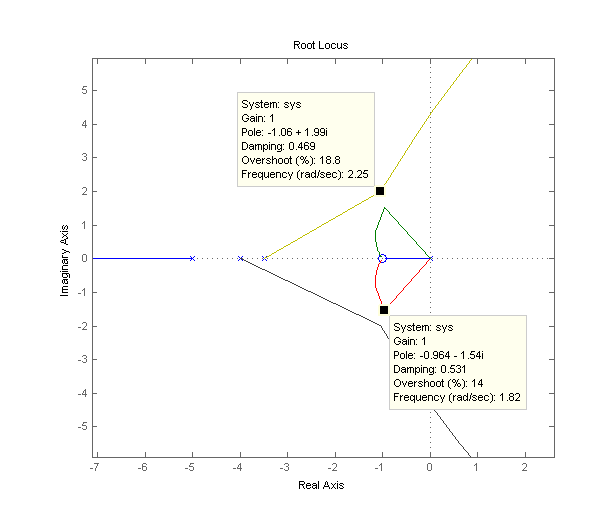
\includegraphics[width=0.80\textwidth]{pics/rlocus}
	\caption{Zoomed root locus plot}
	\label{2:fig:rlocus}
\end{figure}

Two pairs of poles are of primary concern in figure \ref{2:fig:rlocus} above. These are the green/red and yellow/black pairs. These poles are the primary determinant of the overshoot percentage and settling time of the entire control system. These pole pairs will be referred to as the narrow (close to real axis) and wide pairs, respectively.

In order to determine and test the effects of adjusting the gearing ratio (effective torque) on the motor, the motor gear ratio was modified and the root locus was plotted for several values (using the same gain and controller transfer function). It was found that increasing the gearing ratio moved the wide pole pair closer to the real axis and farther to the left in the S-plane. Doing so also increased the imaginary component in the narrow pole pair and moved it closer to the j$\omega$ axis. The gearbox was selected after the poles and zeros of the controller were finalized, in order to fine-tune the final locations of the open loop transfer function poles.

The objective we went for in setting the gearing ratio was matching the overshoot amount of the wide pair and narrow pair poles, so that the overall overshoot (the sum of the overshoot from each pair of poles) would be minimal. This also was done to keep the open loop transfer function as stable as possible. The final open loop transfer function root locus is shown below in figure X. More effective motor torque was required to set the poles to the desired location, so the gear ratio was maximized in order to reduce the size of the motor required (as larger motors are more likely to cost more money to implement). The final gear ratio was 465:1.



\subsection{Motor selection}

The motor selection goes more or less hand in hand with the gearbox selection. The smallest possible motor will be selected, because the gearbox is optimized to produce maximum torque. We selected motor 1, because it was the smallest motor that provided the effective torque we wanted. At this point it becomes a question of what is more important, minimizing the gain of the controller (which will consequently reduce the control effort), or selecting a smaller motor. Either one will move the "wide band" poles to the left in the s-plane and closer to their original positions as well as moving the "narrow band" poles to the right in the s-plane.

Choosing the largest motor and highest motor torque will have the effect of minimizing the control effort of the controller. Control effort was maximized in this case (to make the most efficient use of the controller implemented) so that the smallest motor could be selected. This could be substituted for the largest motor at a fairly high gearing ratio and that should require lower control effort to implement.